
%(BEGIN_QUESTION)
% Copyright 2011, Tony R. Kuphaldt, released under the Creative Commons Attribution License (v 1.0)
% This means you may do almost anything with this work of mine, so long as you give me proper credit

When the loop controller in a {\it feedback} control system is tuned too aggressively, it will result in process oscillations.  This is a well-known fact of loop tuning, and indeed is regarded as a reliable indication of overly-aggressive controller action.

{\it Feedforward} control loops, by contrast, cannot create oscillations.  However, it is still possible to have ``too much'' feedforward action in a loop, so that process control quality suffers.

\vskip 10pt

Examine the following P\&ID of a practical feedforward control system on a heat exchanger, complete with ``gain'' and ``bias'' functions to allow the feedforward action to be adjusted:

$$\includegraphics[width=15.5cm]{i04339x01.eps}$$

How would this feedforward control system respond to load changes if it were ``over-tuned'' so that it took {\it too much} corrective action?  What could you do to this system to test the feedforward control response, in order to tell whether or not the magnitude of its corrective action was appropriate?  Identify the specific adjustments that you would make to this feedforward system so that its action was more appropriate, if it were discovered that the feedforward action was too aggressive.

\vskip 20pt \vbox{\hrule \hbox{\strut \vrule{} {\bf Suggestions for Socratic discussion} \vrule} \hrule}

\begin{itemize}
\item{} Determine the appropriate actions ({\it direct} acting or {\it reverse} acting) for each controller shown in this system, labeling all inputs with either ``+'' or ``$-$'' symbols as appropriate to show the correct action for each controller.
\item{} What types of flowmeters are shown in this P\&ID, and how do they work?
\item{} Identify the individual effects of improper {\it gain} adjustment, versus improper {\it bias} adjustment in the feedforward loop.  Are the effects the same for both?  Why or why not?
\item{} Explain what would happen in this process if the liquid flow transmitter failed with a low signal.
\item{} Explain what would happen in this process if the liquid flow transmitter failed with a high signal.
\item{} Explain what would happen in this process if the steam flow transmitter failed with a low signal.
\item{} Explain what would happen in this process if the steam flow transmitter failed with a high signal.
\item{} Explain what would happen in this process if the temperature transmitter failed with a low signal.
\item{} Explain what would happen in this process if the temperature transmitter failed with a high signal.
\item{} Explain what would happen in this process if the flow controller were switched from ``Cascade'' mode to ``Automatic'' mode.
\item{} Explain what would happen in this process if the flow controller were switched from ``Cascade'' mode to ``Manual'' mode.
\item{} Explain what would happen in this process if the temperature controller were switched from ``Automatic'' mode to ``Manual'' mode.
\end{itemize}

\underbar{file i04339}
%(END_QUESTION)





%(BEGIN_ANSWER)

In order to test the effectiveness of feedforward control, we need to perturb the wild variable (in this case, feed flow rate) and watch the PV's response over time on a trend graph, {\it all with the feedback controller in manual mode so that we are only looking at the effects of feedforward}.  If the feedforward action is ``tuned'' properly, there will be little or no effect on the process (controlled) variable.

%(END_ANSWER)





%(BEGIN_NOTES)

Excessive feedforward control will ``overcompensate'' for load changes.  When the load changes in an overly-aggressive feedforward system, the PV will be disturbed in a direction {\it opposite} that of the load's natural influence.  For example, if the feedforward gain in this system were excessive, increases in cold liquid feed flow rate would result in {\it increasing} outlet temperature.

\vskip 10pt

If a test of feedforward control action reveals it to be too aggressive, the appropriate change would be to reduce the value of the gain (multiplier) function.

%INDEX% Control, strategies: feedforward

%(END_NOTES)

